\documentclass{jsarticle}
\usepackage{moreverb}
\usepackage[dvipdfmx]{graphicx}
\usepackage{float}


\title{計算機実習 問題6.6 - ファイゲンバウム定数の評価 補足}
\author{早稲田大学先進理工学部物理学科 B4 藤本將太郎}
\date{2014/05/05}

\begin{document}

\maketitle

\section{補足}

\begin{enumerate}
 \renewcommand{\labelenumi}{\alph{enumi}.}
 \renewcommand{\labelenumii}{}

 \item 作成したプログラムを使って、$\delta_{k}=(b_{k}-b_{k-1})/(b_{k+1}-b_{k})$を$k$に対してプロットし、$\delta$を求めよ。$b_{k}$の表\ref{tab:t1}に与えられた値の桁数はどの$k$についても十分か。最も精度よく求められている$\delta$の値は
 
 \begin{equation}
  \delta = 4.669\ 201\ 609\ 102\ 991 \cdots
  \label{eq:e2}
 \end{equation}

 である。式(\ref{eq:e2})の小数点以下の桁は、$\delta$が高い精度で求められていることを示している。式(\ref{eq:e1})、式(\ref{eq:e2})および$b_{k}$の値を使って$r_{\infty}$の値を求めよ。

 
  \begin{enumerate}
   \item まず、$\delta_{k}=(b_{k}-b_{k-1})/(b_{k+1}-b_{k})$を$k$に対してプロットしたグラフを、図\ref{fig:f1}に示した。ここで単純に全体の相加平均を求め、その結果を直線にしてグラフに描いた。また、表\ref{tab:t1}に与えられた$b_{k}$の桁数について、$b_{k}$の間隔が$k$が大きくなるにつれて減少していくことを考えると、$b_{8}$の桁数などは十分であるとは言えないだろう。実際、平均値として得られた$\delta$が、精度よく求められている$\delta$の値に近いのに対して、本来$k$が大きいところでは収束するはずの$\delta_{k}$が、そこからずれた値となっていることも、$b_{8}$などの桁数が不足していることを表していると言える。\\
   次に、最小2乗法により式(\ref{eq:e1})におけるパラメータ$c$、$r_{\infty}$を求め、その結果を表\ref{tab:t2}に示す。ここで、得られた値$r_{\infty}=0.892 546 164 091$は非常に正確に調べられていて、その値は$r_{\infty}=0.892 486 417 967 \cdots$である。すなわち、得られた$r_{\infty}$はよく知られている値に対してわずか約0.007%の誤差で精度よく求めることができていることがわかる。

   \begin{figure}[H]
    \begin{center}
     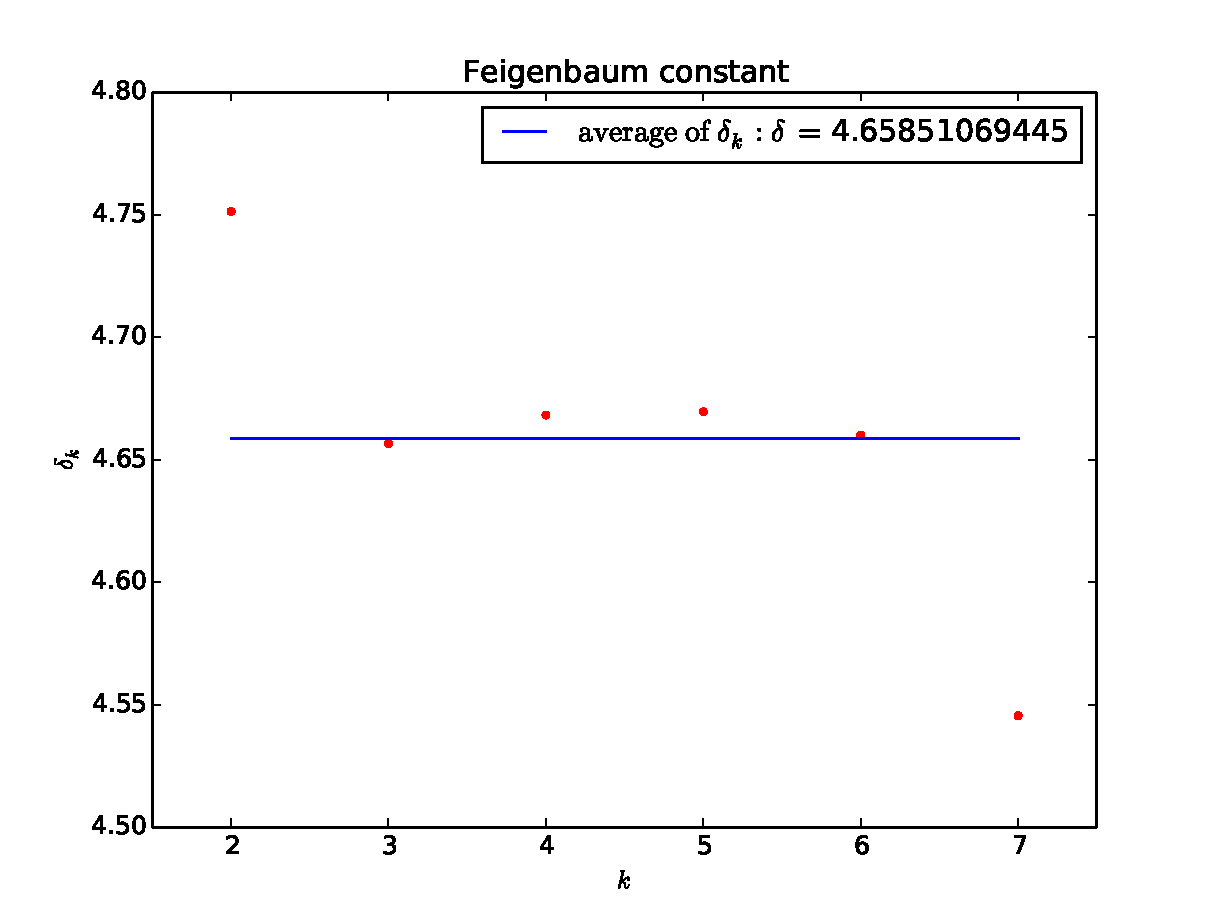
\includegraphics[width=12.0cm]{figure_1.pdf}
     \caption{$\delta_{k}$を$k$に対してプロットしたグラフ}
     \label{fig:f1}
    \end{center}
   \end{figure}
   
   \begin{table}[htbp]
    \begin{center}
     \caption{最小2乗法によって式(\ref{eq:e1})にフィッティングした時のパラメータの値}
     \begin{tabular}{cc}
      パラメータ & 値  \\ \hline
	$c$ & 0.665237682254 \\
	$r_{\infty}$ & 0.892546164091 \\
	\hline
     \end{tabular}
     \label{tab:t2}
    \end{center}
   \end{table}
   
  \end{enumerate}
\end{enumerate}

\section{参考文献}
\begin{itemize}
 \item ハーベイ・ゴールド,ジャン・トボチニク,石川正勝・宮島佐介訳『計算物理学入門』,ピアソン・エデュケーション, 2000.
\end{itemize}

\end{document}
